\section{Conventions de code}
	Par soucis de réutilisabilité et de partage de notre projet, 
	nous avons choisi d'utiliser l'anglais pour la documentation du code mais aussi 
	pour le code en lui-même (noms de fonctions, noms de variables, etc).


\section{Répartition du travail}
	La répartition du travail nous a été indirectement imposé par la structure du projet. 
	
	Tout d'abord la partie analyse du projet s'est faite par le groupe entier car
	c'est une étape fondamentale dans l'élaboration d'un projet. Nous avons donc choisi de
	la faire tous ensemble pour essayer d'avoir une analyse groupée représentative
	et plus poussée. 
	Le projet étant divisé en deux parties, la partie développement \gls{android}
	et la partie \gls{ios}, nous nous sommes repartis de la manière suivante.
	Etant donné que seulement Kilian Cousein et Benjamin Tardieu possédaient un
	Macintosh, ces derniers ont développé la partie iOS. L'autre partie a été
	développé par Olivier Bonvila et Ludovic Pitiot. 
	Enfin en ce qui concerne la partie serveur, c'est Ludovic Pitiot qui l'a implémenté.
	
	
\section{Gestion du projet}
	Afin de garder notre projet cohérent et par soucis de sécurité, nous avons
	choisi de le stocker sur les serveurs de \gls{google_code}. Il y est mis
	gratuitement à disposition des gestionnaires de versions(\gls{svn}), dont voici
	l'adresse de notre projet \url{http://code.google.com/p/bomberman-android-ios/}. 
	Nous avons aussi utilisé le wiki et le gestionnaire de problèmes fournis par
	\gls{google_code}.
	
	Les gestionnaires de versions comme leur nom l'indique, permettent d'avoir à
	porté de main toutes les versions qu'il y a eu d'un fichier depuis sa
	création. Cela permet donc de pouvoir revenir en arrière si une erreur a été
	commise. De plus grâce à cela, notre projet reste cohérent dans le sens où
	pour pouvoir être mis à jour, il faut à tout prix avoir modifié un fichier à
	partir de la dernière version de celui-ci.
		
	Le dernier avantage d'avoir utilisé un gestionnaire de version et qu'il est
	hébergé sur internet et donc chaque membre de l'équipe peut y accéder où qu'il
	soit. 
		
	De plus \gls{google_code} met aussi à disposition de ses utilisateurs des \glspl{wiki}.
	Un \gls{wiki} est un site Web dont les pages sont modifiables par les développeurs
	afin de permettre l'écriture et l'illustration collaborative des documents numériques qu'il contient.
	
	De nombreuses réunions quotidiennes afin d'organiser au mieux le développement
	de cette application, dont nous ignorions tout, ont été faite.
	Nous avons utilisé le \gls{wiki} qui nous a été fourni afin de partager au mieux les découvertes que nous faisions au fur
	et à mesure, ainsi que les articles qui nous semblaient interressants.
	
	En revanche dès lors que nous n'étions pas disponibles ou que nous avions des
	problèmes, Gmail et son chat, se sont avérés indispensables.
	

\section{Gestion du temps}
	La réalisation de notre projet se divise en trois axes. Voilà les différents diagrammes de Gantt de ces derniers.
	
	\subsection*{Organisation}
		\begin{center}
			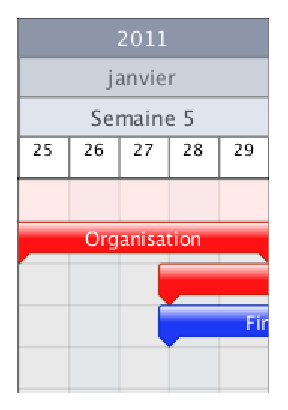
\includegraphics{./Organisation/Img/BomberBlok-Organisation.eps}
		\end{center}
	
	\subsection*{Conception}
		\begin{center}
			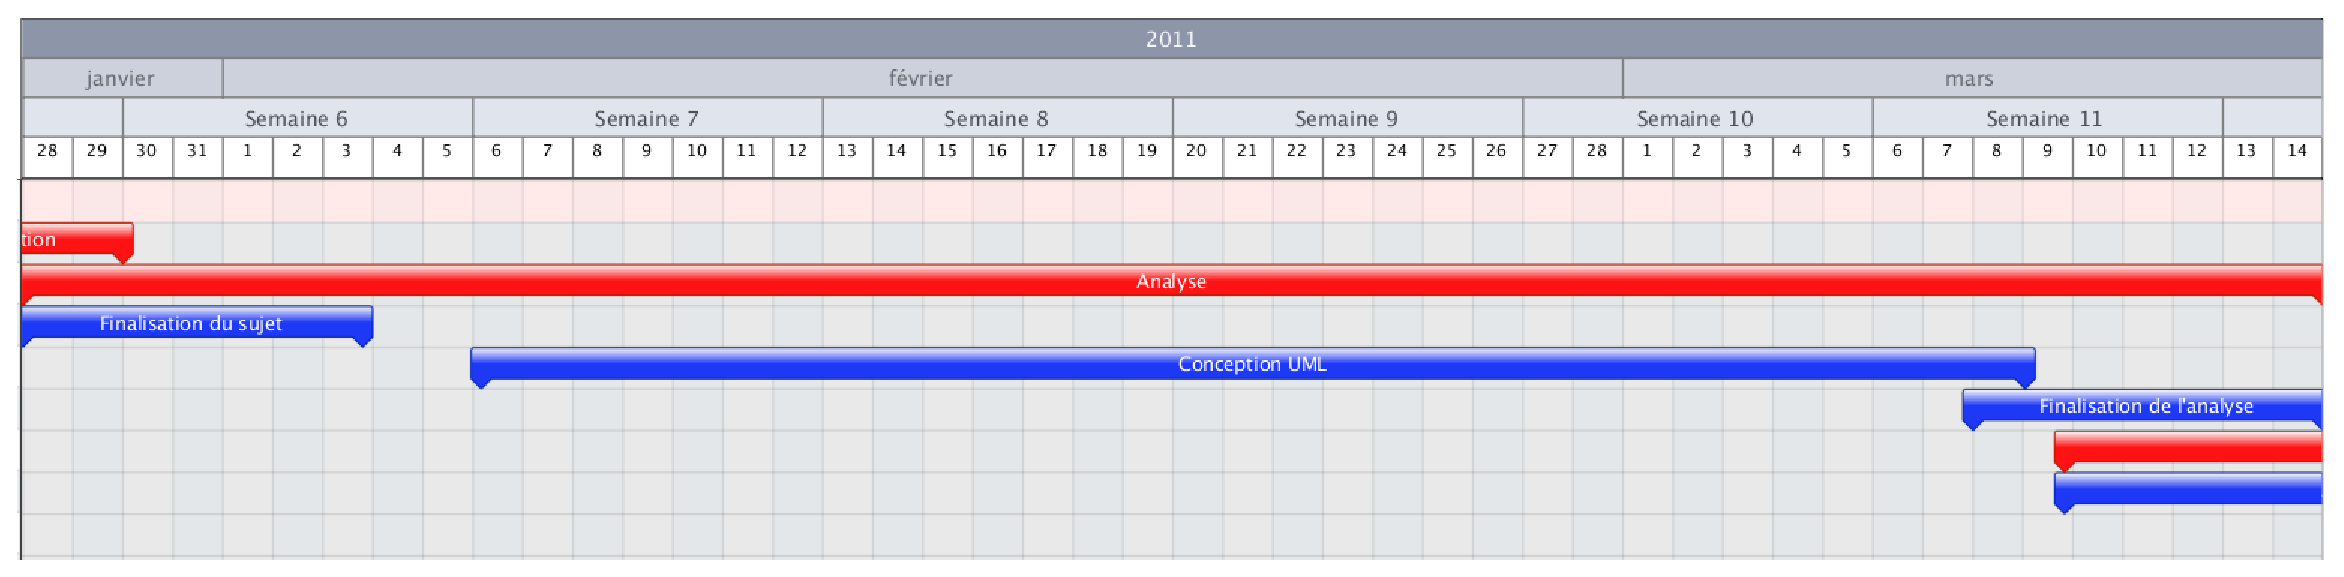
\includegraphics[width=20cm, angle=90]{./Organisation/Img/BomberBlok-Conception.eps}
		\end{center}
	
	\subsection*{Développement}
		\begin{center}
			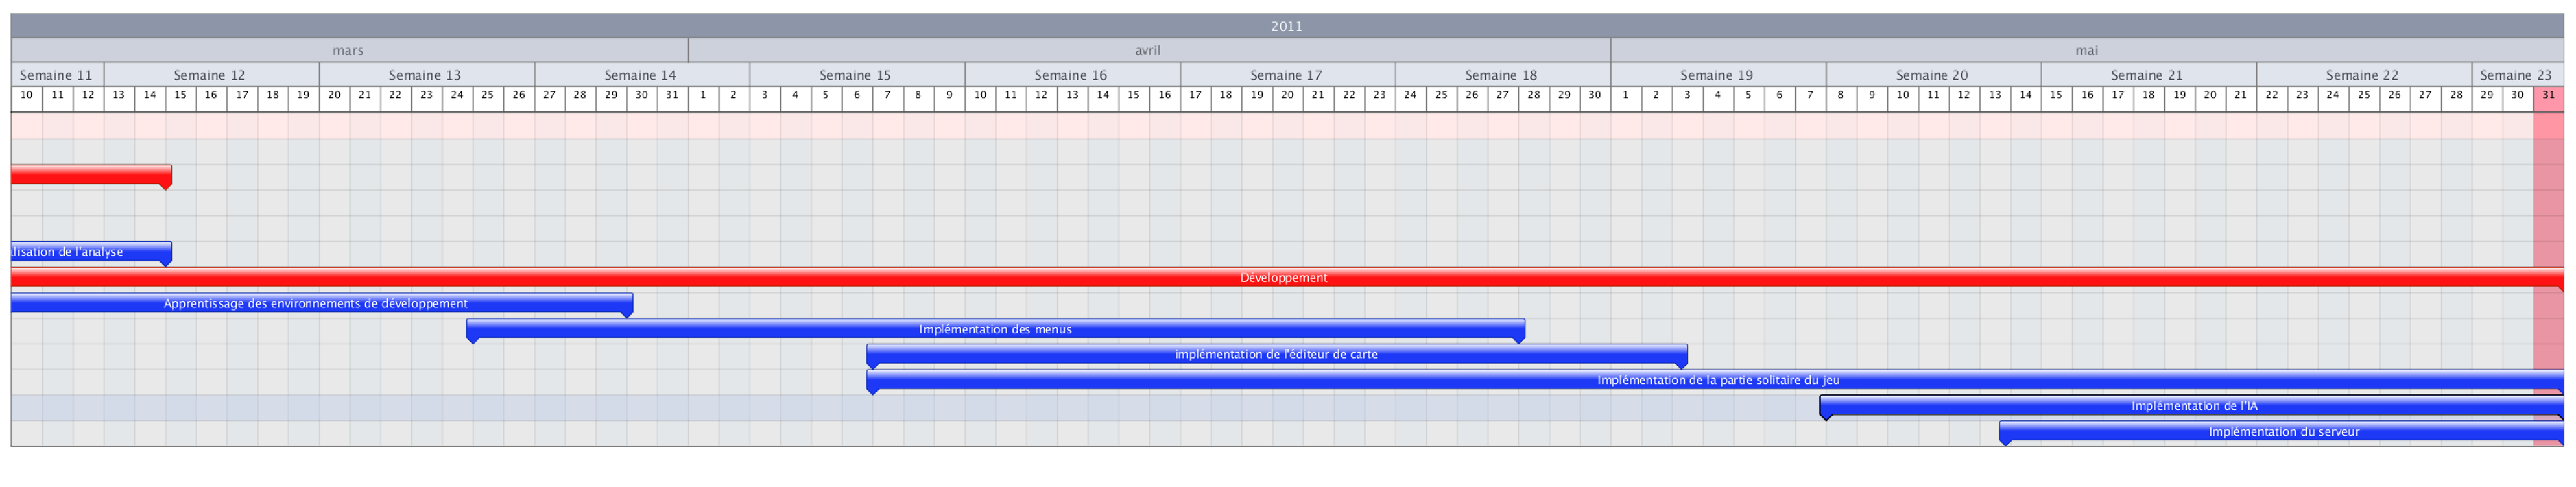
\includegraphics[width=20cm, angle=90]{./Organisation/Img/BomberBlok-Developpement.eps}
		\end{center}
